\documentclass[12pt,a4paper]{article}
\usepackage[utf8]{inputenc}
\usepackage[portuguese]{babel}
\usepackage{amsmath}
\usepackage{graphicx}
\usepackage{geometry}
\geometry{a4paper, margin=2.5cm}
\usepackage{hyperref}
\usepackage{float}
\usepackage{tikz}
\usetikzlibrary{shapes.geometric, arrows.meta, positioning}

\begin{document}

% ==========================================
% CAPA DO RELATÓRIO (Idêntica à Fase 1)
% ==========================================
\begin{titlepage}
    \begin{center}
        % Logo da Universidade
        
\includegraphics[width=5cm]{images/logo_uminho.png}

        \vspace{1cm}
        {\Huge \textbf{Projeto CG}} \\[0.4cm]
        {\large Grupo TP-06} \\[0.2cm]
        {\large Universidade do Minho} \\
        {\large Licenciatura em Engenharia Informática} \\
        {\large Computação Gráfica - 2025/26}
        \vspace{1.5cm}

        \vspace{1.5cm}

        % Fotos dos elementos do grupo
        \begin{minipage}{0.23\textwidth}
            \centering
            
\includegraphics[width=3cm,height=3cm]{images/foto_goncalo.jpeg} \\
            Gonçalo Costa \\ \texttt{A107381}
        \end{minipage}
        \hspace{0.5cm}
        \begin{minipage}{0.23\textwidth}
            \centering
            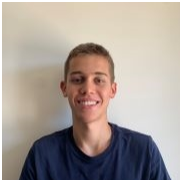
\includegraphics[width=3cm,height=3cm]{images/foto_diogo.jpeg} \\
            Diogo Costa \\ \texttt{A107328}
        \end{minipage}
        \hspace{0.5cm}
        \begin{minipage}{0.23\textwidth}
            \centering
            
\includegraphics[width=3cm,height=3cm]{images/foto_lourenco.jpeg} \\
            Lourenço Martins \\ \texttt{A106849}
        \end{minipage}
        \hspace{0.5cm}
        \begin{minipage}{0.23\textwidth}
            \centering
            
\includegraphics[width=3cm,height=3cm]{images/foto_sa.jpeg} \\
            Gonçalo Sá \\ \texttt{A107376}
        \end{minipage}

        \vfill
        \textbf{\today}
    \end{center}
\end{titlepage}

\tableofcontents
\newpage

% ==========================================
% 1. INTRODUÇÃO
% ==========================================
\section{Introdução} 
O presente relatório detalha o desenvolvimento da segunda fase do projeto da unidade curricular de Computação Gráfica. Esta fase teve como principal objetivo a introdução de transformações geométricas hierárquicas e a criação de grafos de cena (Scene Graphs), permitindo a instanciação e manipulação de múltiplos modelos 3D de forma independente.

Para testar as funcionalidades implementadas, o grande desafio prático desta fase consistiu na modelação de um Sistema Solar dinâmico e hierárquico. Adicionalmente, e como elementos extra de valorização do projeto, o nosso gerador de primitivas foi expandido para suportar uma nova figura geométrica (o Torus, essencial para a representação dos anéis de Saturno), e foi implementado um sistema de navegação de câmara baseado em coordenadas esféricas totalmente controlável através do rato.
% ==========================================
% 2. MOTOR
% ==========================================
\section{Motor} 

\subsection{Estruturas de dados} 
Para suportar o conceito de transformações hierárquicas, o motor de renderização (\textit{Engine}) foi reestruturado de modo a utilizar um grafo de cena (Scene Graph). A estrutura principal definida foi o \textit{Group}, que representa um nó na nossa árvore n-ária. 

Cada grupo contém três componentes fundamentais:
\begin{itemize}
    \item \textbf{Transformações:} Uma lista ordenada de transformações geométricas (Translação, Rotação e Escala) a serem aplicadas ao grupo.
    \item \textbf{Modelos:} Uma lista de modelos 3D (conjuntos de vértices) que pertencem a este nível da hierarquia.
    \item \textbf{Filhos (Children):} Uma lista de subgrupos que herdarão as transformações do grupo pai, permitindo a criação de relações de dependência espacial (por exemplo, a Lua a orbitar a Terra, que por sua vez orbita o Sol).
\end{itemize}

\begin{figure}[H]
    \centering
    \begin{tikzpicture}[
        node distance=1.5cm and 0.2cm, % Reduzi o distanciamento horizontal base
        box/.style={draw, rectangle, rounded corners, minimum width=3.2cm, minimum height=1cm, align=center, fill=blue!5, font=\sffamily},
        root/.style={box, fill=blue!20, font=\sffamily\bfseries\large},
        arrow/.style={-{Stealth[scale=1.2]}, thick, draw=gray!80}
    ]
        % Nó principal
        \node[root] (group) {Group};

        % Sub-nós (reduzi o xshift para ficarem mais juntos)
        \node[box, below left=of group, xshift=-0.5cm] (transforms) {Transformações \\ \footnotesize (Translação, Rotação, Escala)};
        \node[box, below=of group] (models) {Modelos \\ \footnotesize (Vértices 3D)};
        \node[box, below right=of group, xshift=0.5cm] (children) {Filhos \\ \footnotesize (Sub-Grupos)};

        % Ligações
        \draw[arrow] (group) -- (transforms);
        \draw[arrow] (group) -- (models);
        \draw[arrow] (group) -- (children);

        % Seta recursiva mais apertada e com texto em duas linhas
        \draw[arrow, dashed, draw=blue!60] (children.east) -- ++(0.4cm,0) |- (group.east) 
            node[pos=0.25, right, font=\footnotesize\itshape, text=blue!80, align=left] {Árvore n-ária \\ (Recursividade)};
            
    \end{tikzpicture}
    \caption{Diagrama de blocos ilustrando a estrutura de dados de um nó (\textit{Group}) no Grafo de Cena.}
    \label{fig:scene_graph}
\end{figure}

\subsection{Parsing do ficheiro XML} 
O carregamento da cena gráfica foi totalmente automatizado através da biblioteca \textit{TinyXML-2}. O \textit{parser} foi programado para percorrer o ficheiro XML de forma recursiva.

Ao encontrar uma \textit{tag} de grupo, o sistema recolhe primeiramente as transformações geométricas e a sua ordem de aplicação. Em seguida, extrai os ficheiros dos modelos a carregar em memória. Caso o \textit{parser} detete uma nova \textit{tag} de grupo aninhada, a função chama-se a si própria recursivamente, adicionando o resultado à lista de filhos do grupo atual. Esta abordagem garante que qualquer nível de profundidade na árvore do XML seja suportado e lido corretamente para a estrutura em memória.

\subsection{Desenho} 
O processo de desenho (renderização) ocorre através da travessia em profundidade (Depth-First Search) da árvore de grupos. Para garantir que as transformações de um grupo não afetam incorretamente outros grupos adjacentes (irmãos), fazemos uso das funções da API OpenGL para isolamento de matrizes.

Antes de desenhar um grupo, a matriz de transformação atual é guardada na pilha. De seguida, são aplicadas todas as transformações geométricas locais na ordem lida. Após desenhar os modelos pertencentes ao grupo, o motor itera sobre todos os subgrupos, chamando a função de desenho recursivamente. No final, a matriz de transformação original é reposta, garantindo que o estado gráfico retrocede ao do grupo pai.
\subsection{Navegação e Câmara Esférica Orbital} 
Para proporcionar uma exploração mais intuitiva e detalhada das cenas complexas, o motor foi enriquecido com um sistema de navegação baseado numa câmara esférica orbital. Ao contrário de uma câmara estática convencional, esta foca-se num ponto alvo (o \textit{lookAt}) e orbita em torno dele, permitindo inspecionar modelos individuais com grande precisão.

As interações foram mapeadas no motor da seguinte forma:
\begin{itemize}
    \item \textbf{Botão Esquerdo do Rato (Tracking):} Permite a rotação da câmara em torno do ponto alvo atual. O arrastamento horizontal altera o ângulo $\alpha$ (longitude), enquanto o arrastamento vertical altera o ângulo $\beta$ (latitude). Para evitar o \textit{gimbal lock} e a inversão da perspetiva, o ângulo $\beta$ foi restrito ao intervalo de $[-85^\circ, 85^\circ]$.
    \item \textbf{Botão Direito do Rato (Zoom):} Controla a aproximação e o afastamento em relação ao ponto alvo, alterando diretamente a variável do raio ($r$), existindo uma proteção para impedir que o raio seja inferior a $1.0$.
    \item \textbf{Setas Direcionais:} Realizam o \textit{panning} horizontal do sistema, deslocando ativamente as coordenadas X e Z do ponto alvo (\textit{lookX} e \textit{lookZ}).
    \item \textbf{Teclas 'w' e 's':} Realizam o \textit{panning} vertical, subindo e descendo a cota do ponto alvo no eixo Y (\textit{lookY}).
    \item \textbf{Tecla 'x':} Adicionada como um atalho visual para alternar (ligar/desligar) a renderização dos eixos coloridos de referência da cena.
\end{itemize}

A nível de implementação, durante o \textit{parsing} da configuração XML, o motor calcula de forma autónoma o raio e os ângulos iniciais ($\alpha$ e $\beta$) calculando o vetor entre a posição da câmara e o ponto de \textit{lookAt} fornecidos. Durante o ciclo de vida da aplicação, a posição final da câmara é sistematicamente recalculada somando o deslocamento do alvo à conversão esférica:

\begin{align}
    camX &= lookX + r \sin(\alpha) \cos(\beta) \\
    camY &= lookY + r \sin(\beta) \\
    camZ &= lookZ + r \cos(\alpha) \cos(\beta)
\end{align}
% ==========================================
% 3. SISTEMA SOLAR
% ==========================================
\section{Sistema Solar} 

\subsection{Anel de Saturno (Torus)} 
Para representar os anéis de Saturno, foi implementada uma nova primitiva no \textit{Generator}: o \textit{Torus}. O Torus é uma superfície de revolução gerada pela rotação de um círculo ao longo de uma trajetória circular maior.

O algoritmo divide a figura em anéis (\textit{rings}) e fatias (\textit{slices}). As coordenadas cartesianas de cada vértice no espaço 3D são obtidas através das seguintes equações paramétricas:

\begin{align}
    x &= (R + r \cos(v)) \cos(u) \\
    y &= r \sin(v) \\
    z &= (R + r \cos(v)) \sin(u)
\end{align}

Onde:
\begin{itemize}
    \item $R$ corresponde ao raio principal da figura (distância do centro do tubo ao centro global).
    \item $r$ corresponde ao raio do tubo (espessura do anel).
    \item $u \in [0, 2\pi]$ representa o ângulo da secção atual ao longo do eixo Y (\textit{slices}).
    \item $v \in [0, 2\pi]$ representa o ângulo em torno do tubo (\textit{rings}).
\end{itemize}
Durante a implementação desta primitiva no gerador, houve um cuidado acrescido na definição dos vértices para garantir que a \textit{Winding Order} (ordem de desenho dos triângulos) respeitava o sentido anti-horário (\textit{Counter-Clockwise}). Esta precaução matemática revelou-se fundamental para assegurar a total compatibilidade do modelo com a funcionalidade de \textit{Backface Culling} ativada no motor, otimizando a renderização final.
\begin{figure}[H]
    \centering
    \begin{tikzpicture}[>=stealth, scale=1.2]
        % Variáveis base
        \def\R{4.5}  % Raio principal R 
        \def\r{1.3}  % Raio do tubo r

        % Eixos globais (X, Y, Z)
        \draw[->, thick, gray] (0,0) -- (0,3) node[above, text=black] {$Y$};
        \draw[->, thick, gray] (0,0) -- (-2.5,-1.5) node[below left, text=black] {$Z$};
        \draw[->, thick, gray] (0,0) -- (7.5,0) node[right, text=black] {$X$};

        % Elipse base para simular a trajetória 3D do anel central
        \draw[dashed, thick, blue!40] (0,0) ellipse ({\R} and {\R*0.3});

        % Ângulo u (Slices) em torno do eixo Y
        \draw[->, thick, blue] (2.5,0) arc (0:140:2.5 and 0.75) 
            node[pos=0.6, above right, align=center, text=blue!90!black, fill=white, inner sep=1pt] {Ângulo $u$ \\ (\textit{slices})};

        % Centro do círculo transversal (Tubo) no eixo X
        \coordinate (C) at (\R, 0);

        % Círculo transversal (Representa o Tubo)
        \draw[thick, fill=red!5, draw=red!60!black] (C) circle (\r);
        
        % Pontos e legendas principais
        \filldraw[black] (C) circle (1.5pt) node[below=4pt, font=\footnotesize, text=black] {Centro do tubo};
        \filldraw[black] (0,0) circle (1.5pt) node[above left=2pt, font=\footnotesize, text=black] {Origem};

        % Cotação do Raio principal R
        \draw[dashed, gray] (0,0) -- (0, -2);
        \draw[dashed, gray] (C) -- (\R, -2);
        \draw[<->, thick, blue!80!black] (0, -1.8) -- (\R, -1.8) 
            node[midway, fill=white, inner sep=3pt] {$R$ (Raio principal)};

        % Cotação do Raio do tubo r 
        \draw[<->, thick, red!80!black] (C) -- ++(135:\r) node[midway, below left=1pt, fill=white, inner sep=1pt] {$r$};

        % Linha auxiliar para o ângulo v (estendida para fora)
        \draw[dashed, thin, gray] (C) -- ++(0:\r+1);

        % Ângulo v (Rings) em torno do tubo - Desenhado pelo LADO DE FORA do tubo (raio 1.6)
        \draw[->, thick, red!80!black] (\R+1.6, 0) arc (0:110:1.6) 
            node[pos=0.5, right=4pt, align=left, text=red!80!black, fill=white, inner sep=2pt] {Ângulo $v$ \\ (\textit{rings})};

    \end{tikzpicture}
    \caption{Esquema paramétrico do Torus desenhado no \textit{Engine}. O ângulo $u$ representa a rotação em torno do eixo $Y$ (\textit{slices}), enquanto $v$ descreve a secção transversal de raio $r$ (\textit{rings}).}
    \label{fig:torus_math}
\end{figure}
\subsection{Modelos utilizados} 
A construção do Sistema Solar dependeu amplamente de duas primitivas geradas na Fase 1 e Fase 2. O Sol e todos os planetas (incluindo as respetivas luas) foram modelados utilizando \textit{Esferas} com variações nos seus raios e níveis de tesselagem. Adicionalmente, utilizou-se a recém-criada primitiva \textit{Torus} para esculpir o anel de Saturno.

\subsection{Formato do ficheiro XML e Transformações} 
O ficheiro XML foi moldado para refletir as distâncias relativas e as translações necessárias para a simulação de órbitas. Para tal, as transformações geométricas foram aplicadas com uma ordem e lógica específicas:
\begin{itemize}
    \item \textbf{Sol e Planetas:} O Sol foi colocado no nó principal, sofrendo apenas uma transformação de Escala. Para cada planeta, foi aplicado primeiramente um ângulo de \textit{Rotação} em torno da origem (eixo Y) para determinar a sua posição orbital, seguido de uma \textit{Translação} no eixo X, que o afasta do centro e define o raio da sua órbita.
    \item \textbf{Sistema Terra-Lua:} A Lua encontra-se num subgrupo da Terra. Graças à herança de matrizes do motor, a Lua herda a translação principal do seu planeta-mãe. Assim, bastou aplicar à Lua uma translação local ligeira (de 2.5 unidades) para a afastar do centro da Terra.
    \item \textbf{Anel de Saturno:} O modelo do \textit{Torus} foi instanciado num subgrupo de Saturno e sofreu uma transformação de \textit{Escala} com um valor reduzido no eixo Y, de modo a achatá-lo e conferir-lhe um aspeto realista de anel planetário.
\end{itemize}

A nível estrutural, a relação "Sol $\rightarrow$ Terra $\rightarrow$ Lua" foi configurada conforme ilustrado no diagrama da Figura \ref{fig:xml_hierarchy}.
\begin{figure}[H]
    \centering
    \begin{tikzpicture}[
        node distance=1.5cm and 2cm,
        group/.style={draw=blue!60, rectangle, rounded corners, minimum width=2.8cm, minimum height=0.8cm, align=center, fill=blue!5, font=\sffamily\bfseries},
        model/.style={draw=green!60!black, rectangle, rounded corners, minimum width=2.5cm, minimum height=0.6cm, align=center, fill=green!5, font=\sffamily\footnotesize},
        arrow/.style={-{Stealth[scale=1.2]}, thick, draw=gray!80}
    ]
        % 1. Grupo Central (Sol)
        \node[group] (sol) {Group (Sol)};
        \node[model, right=1.5cm of sol] (mod_sol) {Modelo: Esfera (Sol)};
        \draw[arrow] (sol) -- (mod_sol);
        
        % 2. Grupo da Terra (Subgrupo do Sol)
        \node[group, below=1.2cm of sol, xshift=2.5cm] (terra) {Group (Terra)};
        \node[model, right=1.5cm of terra] (mod_terra) {Modelo: Esfera (Terra)};
        \draw[arrow] (terra) -- (mod_terra);
        
        % 3. Grupo da Lua (Subgrupo da Terra)
        \node[group, below=1.2cm of terra, xshift=2.5cm] (lua) {Group (Lua)};
        \node[model, right=1.5cm of lua] (mod_lua) {Modelo: Esfera (Lua)};
        \draw[arrow] (lua) -- (mod_lua);
        
        % Ligações Hierárquicas (XML Group dentro de Group)
        % O "pos=0.25" coloca o texto no meio da linha VERTICAL.
        % O "left=3pt" afasta-o ligeiramente para a esquerda.
        \draw[arrow, draw=blue!60] (sol.south) |- (terra.west) 
            node[pos=0.25, left=3pt, font=\footnotesize\itshape, text=blue!80!black, align=right] {Translação \\ (Afasta do Sol)};
            
        \draw[arrow, draw=blue!60] (terra.south) |- (lua.west) 
            node[pos=0.25, left=3pt, font=\footnotesize\itshape, text=blue!80!black, align=right] {Translação \\ (Afasta da Terra)};
            
    \end{tikzpicture}
    \caption{Diagrama hierárquico ilustrando o Grafo de Cena gerado a partir do ficheiro XML. As caixas azuis representam os nós de transformação (\textit{Groups}) e as caixas verdes representam a instanciação das primitivas 3D (\textit{Modelos}).}
    \label{fig:xml_hierarchy}
\end{figure}

\subsection{Resultado final} 
Para a exploração visual da cena hierárquica construída, as interações de câmara esférica desenvolvidas no motor (Secção 2.4) revelaram-se fundamentais. A capacidade de orbitar livremente e ajustar o \textit{zoom} permitiu inspecionar as órbitas dinâmicas do Sistema Solar com grande precisão. Adicionalmente, a alternância entre os modos de desenho (Polígonos preenchidos, Linhas e Pontos) continuou a ser suportada pelas teclas 'f', 'l' e 'p', sendo fulcral para a visualização detalhada das malhas do anel de Saturno.
% --- 1. Sistema Solar: Linhas vs Preenchido ---
\begin{figure}[H]
    \centering
    \begin{minipage}{0.48\textwidth}
        \centering
        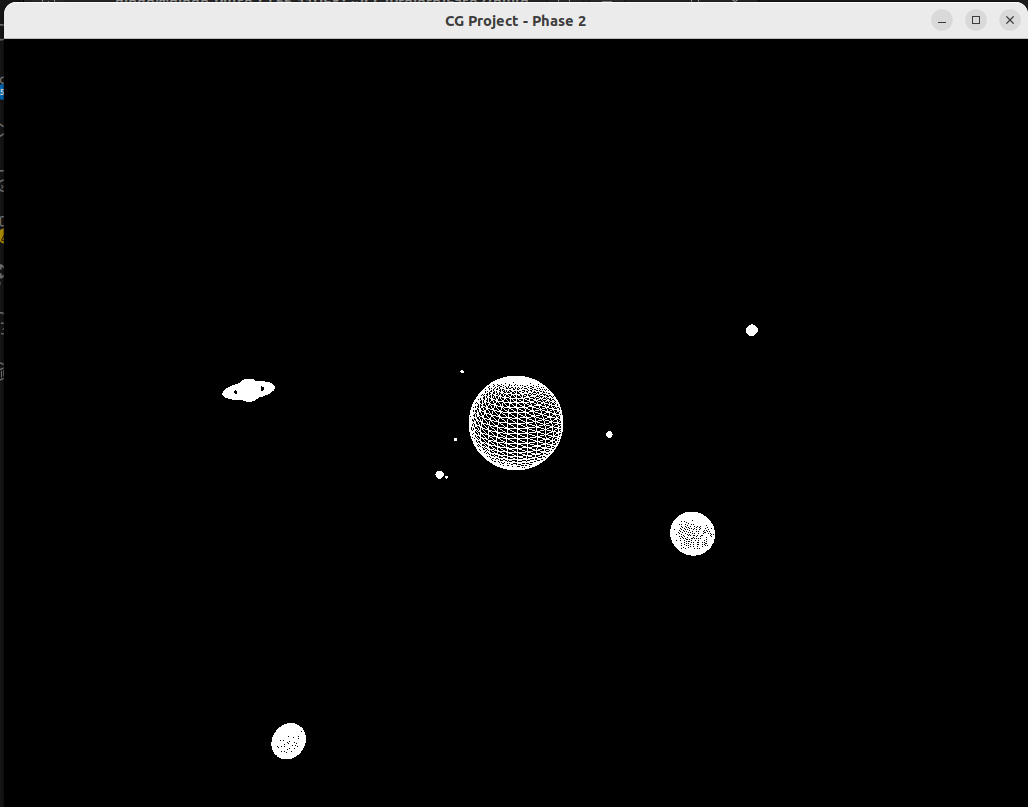
\includegraphics[width=\textwidth]{images/sistema_solar_linhas.png} % <-- Substituir
        \caption{Visão global do Sistema Solar evidenciando as malhas em modo de linhas (\textit{Wireframe}).}
        \label{fig:solar_linhas}
    \end{minipage}\hfill
    \begin{minipage}{0.48\textwidth}
        \centering
        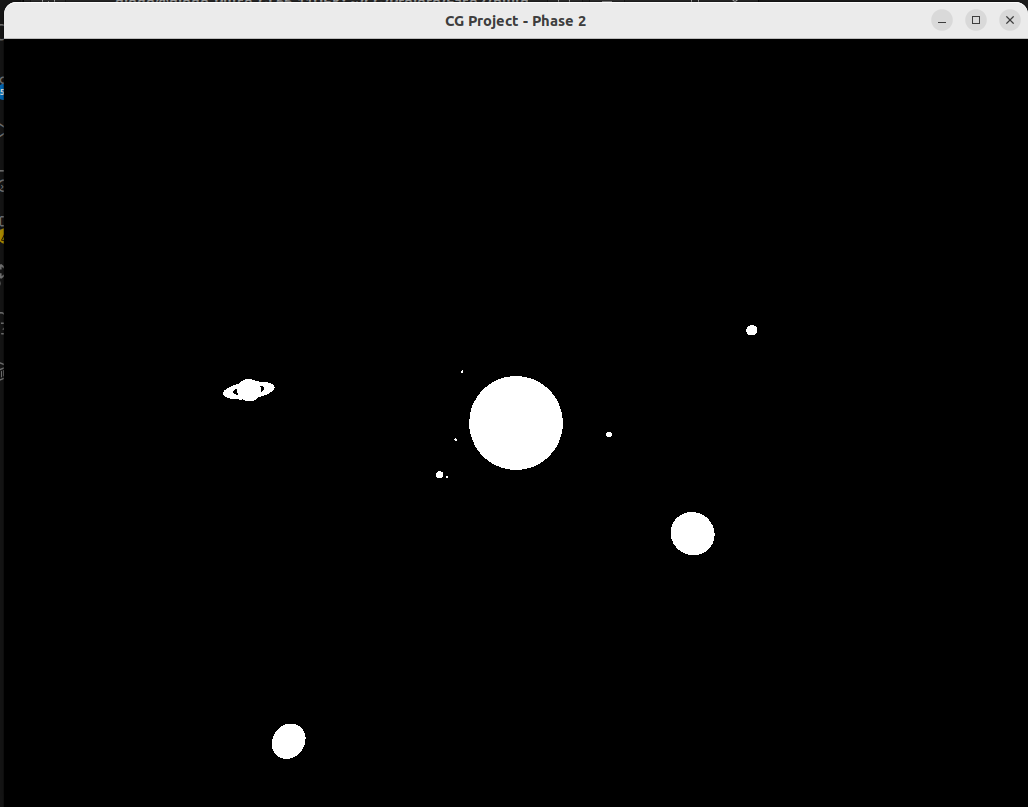
\includegraphics[width=\textwidth]{images/sistema_solar_preenchido.png} % <-- Substituir
        \caption{Visão global do Sistema Solar renderizado com polígonos preenchidos (\textit{Fill}).}
        \label{fig:solar_preenchido}
    \end{minipage}
\end{figure}

% --- 2. Detalhes: Saturno e Terra-Lua ---
\begin{figure}[H]
    \centering
    \begin{minipage}{0.48\textwidth}
        \centering
        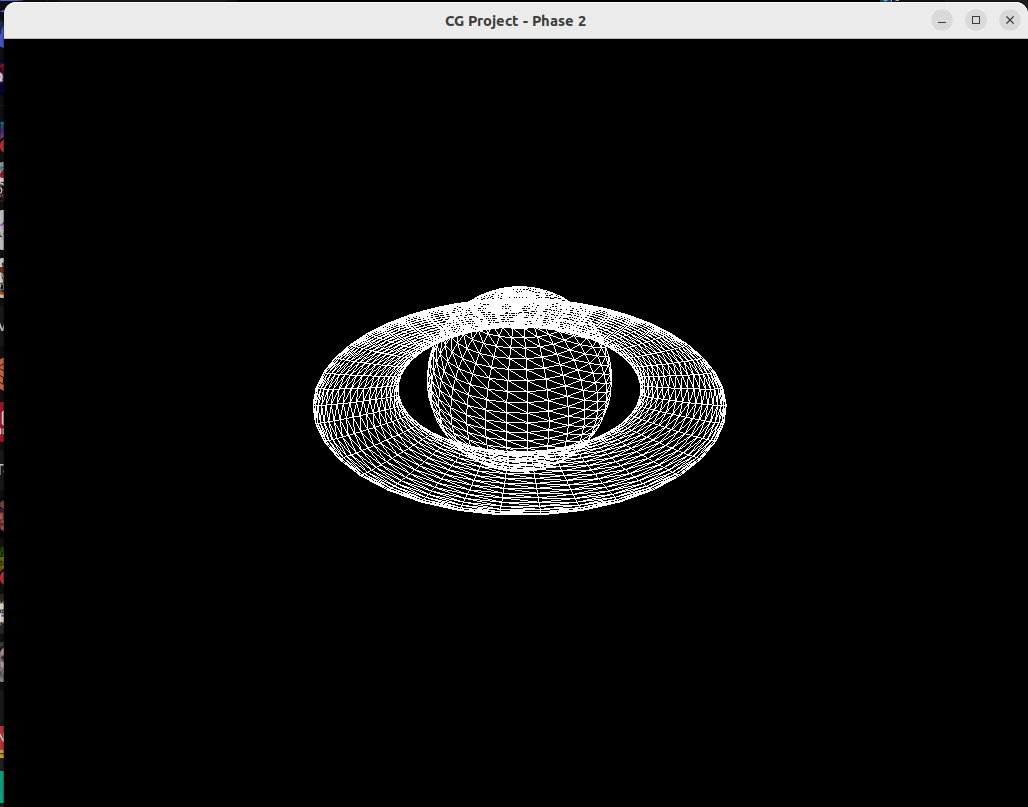
\includegraphics[width=\textwidth]{images/saturno.png} % <-- Substituir
        \caption{Detalhe de Saturno, destacando o anel gerado através da nova primitiva \textit{Torus}.}
        \label{fig:saturno}
    \end{minipage}\hfill
    \begin{minipage}{0.48\textwidth}
        \centering
        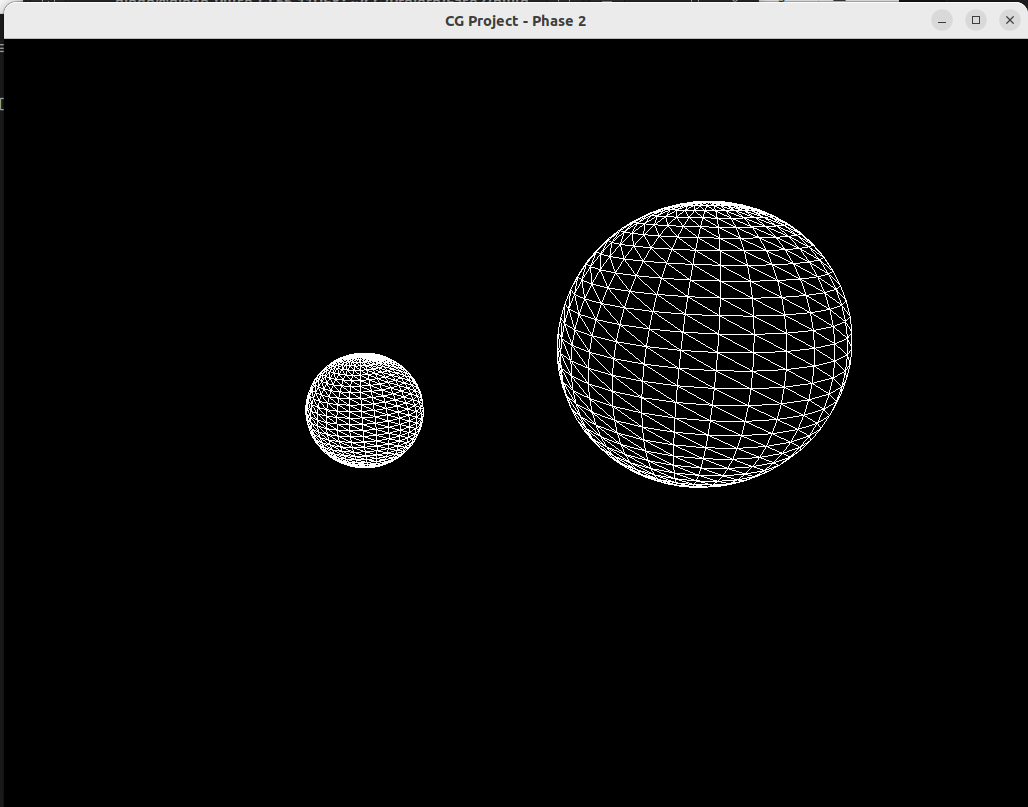
\includegraphics[width=\textwidth]{images/terra_lua.png} % <-- Substituir
        \caption{Detalhe da órbita lunar, validando o isolamento de matrizes no sistema Terra-Lua.}
        \label{fig:terra_lua}
    \end{minipage}
\end{figure}

% --- 3. Resultados dos Ficheiros de Teste (Grelha 2x2) ---
Antes da elaboração da cena final, a integridade do Grafo de Cena e da Pilha de Matrizes foi rigorosamente validada utilizando os ficheiros XML de configuração fornecidos (Cenários de Teste 1 a 4). Esta fase de testes foi essencial para comprovar que as transformações geométricas são aplicadas na ordem correta, que a herança de transformações ocorre sem falhas para os subgrupos descendentes e que os modelos são renderizados nas posições correspondentes às imagens de controlo. Os resultados obtidos podem ser observados na figura abaixo.
\begin{figure}[H]
    \centering
    % Primeira linha dos testes
    \begin{minipage}{0.48\textwidth}
        \centering
        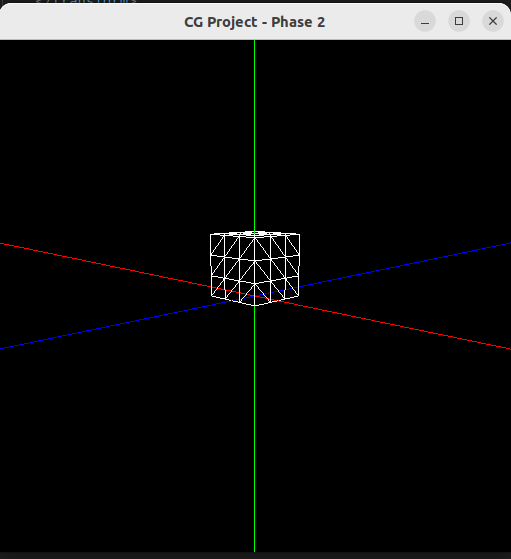
\includegraphics[width=\textwidth]{images/teste1.png} % <-- Substituir (ex: 4_1.png)
        \caption{Renderização do cenário de teste 1.}
        \label{fig:teste1}
    \end{minipage}\hfill
    \begin{minipage}{0.48\textwidth}
        \centering
        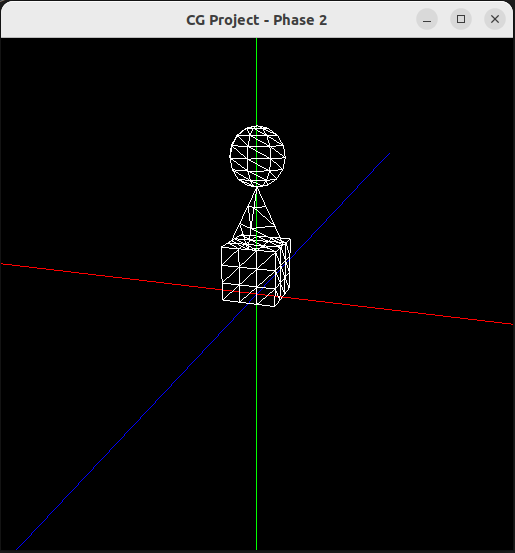
\includegraphics[width=\textwidth]{images/teste2.png} % <-- Substituir (ex: 4_2.png)
        \caption{Renderização do cenário de teste 2.}
        \label{fig:teste2}
    \end{minipage}
    
    \vspace{0.6cm} % Espaçamento vertical entre as linhas da grelha
    
    % Segunda linha dos testes
    \begin{minipage}{0.48\textwidth}
        \centering
        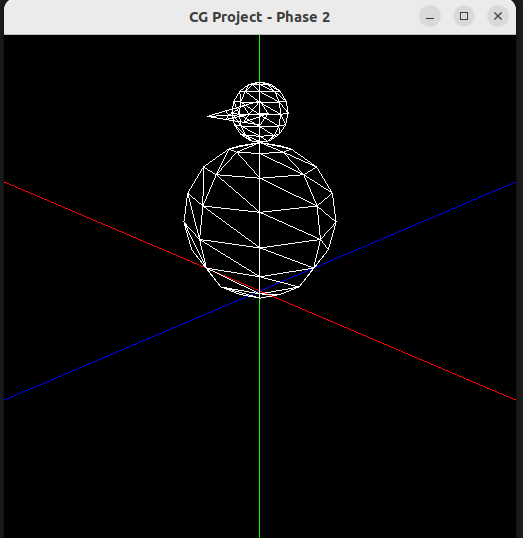
\includegraphics[width=\textwidth]{images/teste3.png} % <-- Substituir (ex: 4_3.png)
        \caption{Renderização do cenário de teste 3.}
        \label{fig:teste3}
    \end{minipage}\hfill
    \begin{minipage}{0.48\textwidth}
        \centering
        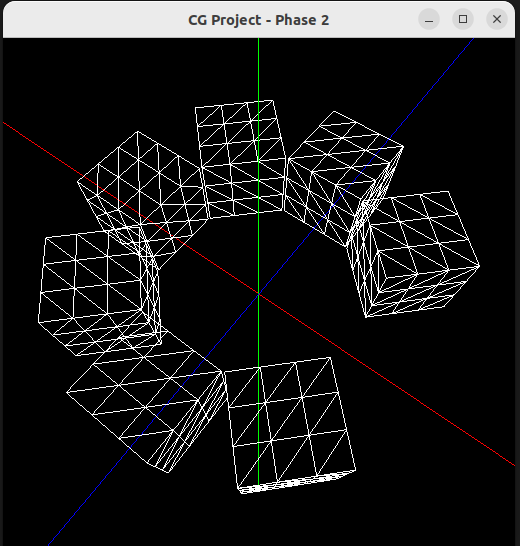
\includegraphics[width=\textwidth]{images/teste4.png} % <-- Substituir (ex: 4_4.png)
        \caption{Renderização do cenário de teste 4.}
        \label{fig:teste4}
    \end{minipage}
\end{figure}

% ==========================================
% 4. CONCLUSÃO
% ==========================================
\section{Conclusão} 
Ao longo desta segunda fase do projeto, a equipa conseguiu consolidar e implementar com sucesso os conceitos de transformações geométricas matriciais e estruturas de dados em árvore.

A passagem de uma renderização estática para um Grafo de Cena hierárquico provou-se totalmente funcional com a apresentação escalável e interativa do Sistema Solar. A modularidade do nosso código no \textit{Engine} e a correta expansão matemática do \textit{Generator} para incluir o Torus deixam o motor gráfico perfeitamente preparado para a adoção de curvas Catmull-Rom e VBOs nas fases seguintes do projeto.

\end{document}